\chapter{INTRODUCCIÓN}
\lipsum[1-3]\cite{herrera2015sliding}.

\section{Objetivo General}
\lipsum[1-3]\cite{herrera2015sliding}.
Realizar el control de un Robot con Arquitectura Antropomórfica de cinco grados de libertad que realice tareas de paletización \cite{chamorro2020high}.

\begin{figure}[H]
    \centering
    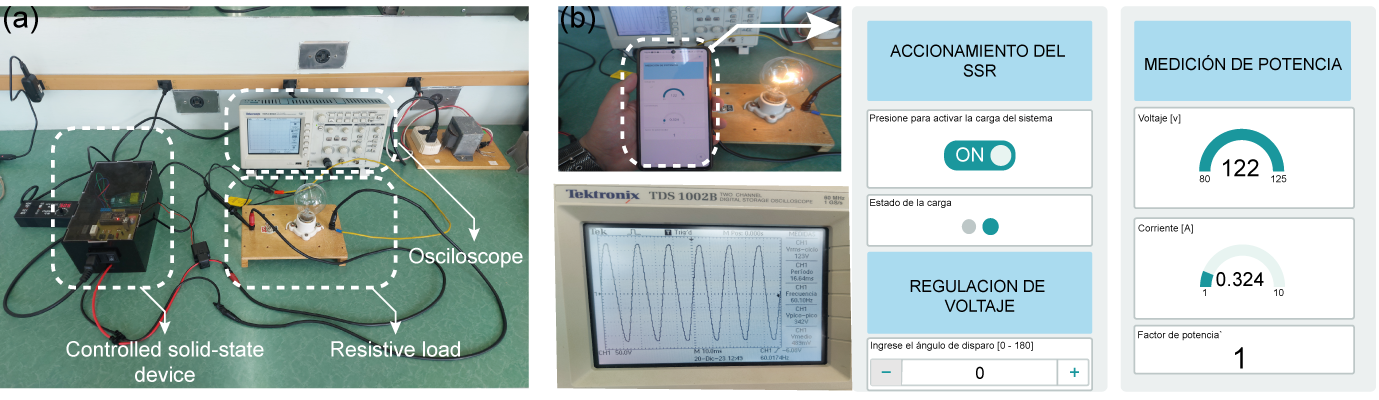
\includegraphics[width=\textwidth]{figuras/testR.png} % Replace with your image file path
    \caption{Gemelo Digital y Gemelo Físico.}
    \label{fig:gemelo_digital}
\end{figure}



\section{Objetivos Específicos}
\begin{itemize}
    \item Realizar revisión bibliográfica del TIC “Ensamblaje y Control de un Robot con Arquitectura Antropomórfica de cinco grados de libertad”.
    \item Adaptar el software de control en alto y bajo nivel para realizar tareas de paletización.
\end{itemize}

\section{Alcance}
Realizar una revisión bibliográfica del diseño del robot antropomórfico de cinco grados de libertad.

\section{Marco Teórico}
Realizar una revisión bibliográfica del diseño del robot antropomórfico de cinco grados de libertad
\subsection{Estado del Arte}

\lipsum[1-3]\cite{herrera2015sliding}.